\chapter{Psalm 14}

\begin{figure}
  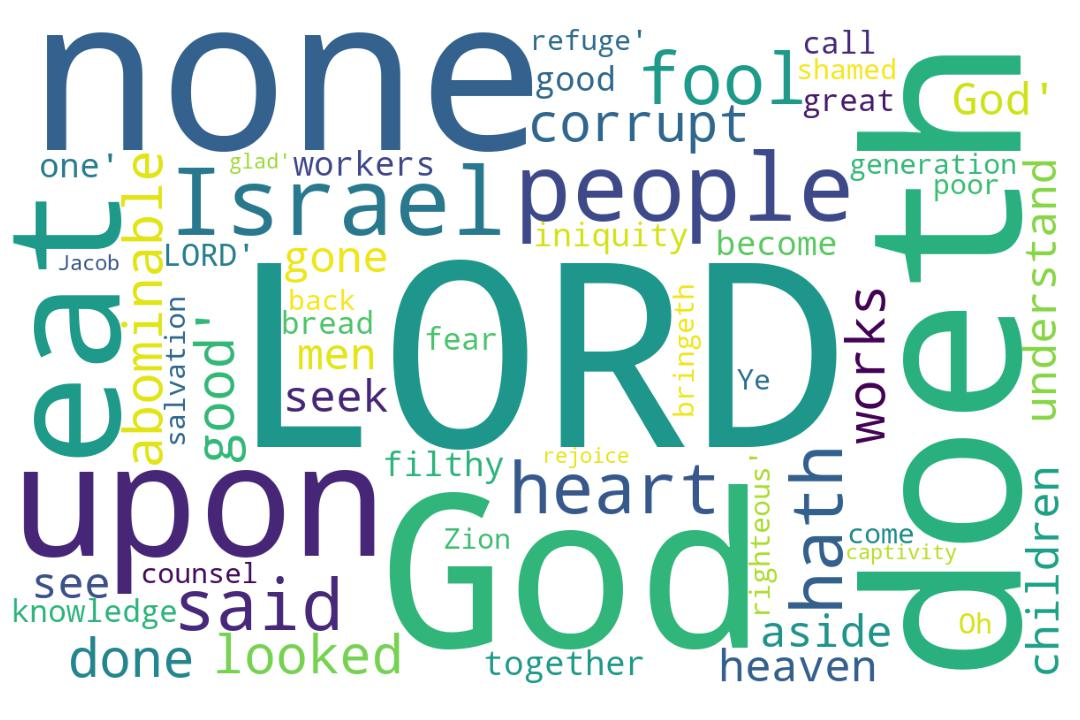
\includegraphics[width=\linewidth]{19OT-Psalms/Psalm14-WordCloud.jpg}
  \caption{Psalm 14 Word Cloud}
  \label{fig:Psalm 14 word Cloud}
\end{figure}



\marginpar{\scriptsize \centering \fcolorbox{bone}{lime}{\textbf{THINGS OF THE WICKED}}\\ (Psalm 14:1-7) \begin{compactenum}[I.][8]
    \item \textbf{Dwelling Place} of the Wicked (Job 08:22) 
	\item\textbf{Foolish Atheists} - They say this because they choose to believe it, as if saying so will make God disappear. It is like the ostrich burying his head in sand - if they can't see God, or won't, then God will go away for them. (Psa 14:1) 
	\item  \textbf{Full Abandonement}  (Psa 14:3)
	\item Man has become \textbf{Filthy Altogether} (Psa 14:3)
	\item Man has developed a \textbf{Fierce Appetite} (Psa 14:4)
	\item But they have a \textbf{Fearful Attitude} (Psa 14:5)
    \item David awaits the \textbf{Final Arrival} (Psa 14:7)
\end{compactenum}}

\marginpar{\scriptsize \centering \fcolorbox{bone}{yellow}{\textbf{LANGUISHING AND LONGING}}\\ (Psalm 14:1-7) \begin{compactenum}[I.][8]
    \item \textbf{Foul Activities} (Psa 14:1) 
	\item\textbf{Foolish Atheists} - They say this because they choose to believe it, as if saying so will make God disappear. It is like the ostrich burying his head in sand - if they can't see God, or won't, then God will go away for them. (Psa 14:1) 
	\item  \textbf{Full Abandonement}  (Psa 14:3)
	\item Man has become \textbf{Filthy Altogether} (Psa 14:3)
	\item Man has developed a \textbf{Fierce Appetite} (Psa 14:4)
	\item But they have a \textbf{Fearful Attitude} (Psa 14:5)
    \item David awaits the \textbf{Final Arrival} (Psa 14:7)
\end{compactenum}}

\footnote{\textcolor[cmyk]{0.99998,1,0,0}{\hyperlink{TOC}{Return to end of Table of Contents.}}}\footnote{\href{https://www.audioverse.org/english/audiobibles/books/ENGKJV/O/Ps/1}{\textcolor[cmyk]{0.99998,1,0,0}{Psalms Audio}}}\textcolor[cmyk]{0.99998,1,0,0}{To the chief Musician, \emph{A Psalm} of David.}\footnote{Ryrie notes that this psalm, with only slight changes in verse 5 and 6, is identical to Psalm 53. \cite{ryrie2008ryrieKJV}
\begin{compactenum}[I.][3]
\item (Psalm 14:1-6) David laments the moral foolishness and corruption of the whole human race  
\item (Psalm 14:7) David  longs for the establishment of the righteous kingdom of the Lord of earth (14:7)
\end{compactenum} }\\
\\
\textcolor[cmyk]{0.99998,1,0,0}{The fool hath said in his heart, \emph{There} \emph{is} no God. They are corrupt, they have done abominable works, \emph{there} \emph{is} none that doeth good.}\footnote{From Kidner, the spirit of godlessness reveals itself in two ways:  in flouting God's law (1-3) and oppressing His people (4-6); that is, in both direct and indirect contempt of heaven. It is the reckless folly (1a,2b, 4a) almost as much as the wickedness of it that energes in the psalm, which `looks down from heaven' on the scene as God views it. But the standpoint changes in the last verse to the earthly arena, where persecuted Israel waits longingly for the redress that will surely come. The psalm is almost exactly duplicated in Psalm 53, where, however, the term `God' replaces `The Lord'. \cite{kidner2014psalmsV1} } 
[2] \textcolor[cmyk]{0.99998,1,0,0}{The LORD looked down from heaven upon the children of men, to see if there were any that did understand, \emph{and} seek God.}\footnote{\textbf{Psalm 11:4} - The LORD is in his holy temple, the LORD'S throne is in heaven: his eyes behold, his eyelids try, the children of men.}\footnote{\textbf{Psalm 33:13} - The LORD looketh from heaven; he beholdeth all the sons of men.}\footnote{\textbf{Psalm 102:19} - For he hath looked down from the height of his sanctuary; from heaven did the LORD behold the earth;}
[3] \textcolor[cmyk]{0.99998,1,0,0}{They are all gone aside, they are \emph{all} together become filthy: \emph{there} \emph{is} none that doeth good, no, not one.}\footnote{\textbf{Romans 3:10-12} - }
[4] \textcolor[cmyk]{0.99998,1,0,0}{Have all the workers of iniquity no knowledge? who eat up my people \emph{as} they eat bread, and call not upon the LORD.}%\footnote{These are the people that say you cannot correct “the Hebrew’’ with the English. These are the people who swear by ``plenary, verbally inspired'' scraps of paper that contain a DEAD language on them. These are the people that would call you a ``heretic'' for correcting their banal, benighted, bewildered, tedious, misinformed BUNKO with the Authorized Version. Had enough? Ready for some Scripture instead of the ``original Hebrew''? \begin{compactenum}
%\item People in the Bible EAT people (Lam. 4:10; Deut. 28:53–56; 2 Kings 6:29). Is that clear? Do you understand that?
%\item Dragons eat people (Jer. 51:34). Do you understand that?
%\item Israelites will be eaten (Isa. 6:13). Do you understand THAT?
%\item Someone goes after a Jew to eat his flesh (Ps. 27:2).
%\item Someone who professed to drink literal blood every Sunday morning at eleven o’clock, offers drink offerings of blood (Ps. 16:4). Any trouble yet?
%\item When you sacrifice at an altar, you cut off the head of the victim (Lev. 1:12). When you sacrifice people (Rev. 6:9) you cut off their heads (Rev. 20:4). Any problem? What is the problem?
%\end{compactenum} }
\footnote{\textbf{Psalm 27:2} -- When the wicked, even mine enemies and my foes, came upon me to eat up my flesh, they stumbled and fell.}
[5] \textcolor[cmyk]{0.99998,1,0,0}{There were they in great fear: for God \emph{is} in the generation of the righteous.}
[6] \textcolor[cmyk]{0.99998,1,0,0}{Ye have shamed the counsel of the poor, because the LORD \emph{is} his refuge.}\footnote{\textbf{Psalm 9:9} - The LORD also will be a refuge for the oppressed, a refuge in times of trouble.}\footnote{\textbf{Hebrews 6:18} - That by two immutable things, in which it was impossible for God to lie, we might have a strong consolation, who have fled for refuge to lay hold upon the hope set before us:}\footnote{\textbf{Psalm 22:30} -- A seed shall serve him; it shall be accounted to the Lord for a generation.}\footnote{\textbf{Psalm 24:6} - This is the generation of them that seek him, that seek thy face, O Jacob. Selah.}\footnote{\textbf{PSalm 73:15} - If I say, I will speak thus; behold, I should offend against the generation of thy children.}\footnote{\textbf{Psalm 112:2} - His seed shall be mighty upon earth: the generation of the upright shall be blessed.}\footnote{\textbf{1 Peter 2:9} - But ye are a chosen generation, a royal priesthood, an holy nation, a peculiar people; that ye should shew forth the praises of him who hath called you out of darkness into his marvellous light:}
[7] \textcolor[cmyk]{0.99998,1,0,0}{Oh that the salvation of Israel \emph{were} \emph{come} out of Zion! when the LORD bringeth back the captivity of his people, Jacob shall rejoice, \emph{and} Israel shall be glad.}\footnote{\textbf{Psalm 53:6} - Oh that the salvation of Israel were come out of Zion! When God bringeth back the captivity of his people, Jacob shall rejoice, and Israel shall be glad.}
